% ID: SEL-D0015-BA-E02
% ESTADO: validada. S016. Revisión matemática, didáctica y visual.
\textbf{a) Formulación, sin resolver.}\par\nopagebreak[4]
Sean $x$ e $y$ las horas de funcionamiento de las cadenas A y B. Las horas pueden tomar valores reales no negativos. Se busca
\[
\boxed{\min C(x,y)=1200x+1500y}
\]
sujeto a
\[
\begin{cases}10x+7y\geq400&\text{(lavadoras)},\\5x+6y\geq280&\text{(frigoríficos)},\\x\leq2y&\text{(límite de horas A)},\\x\geq0,\quad y\geq0.\end{cases}
\]
Se conserva ``como mínimo'' mediante desigualdades de sentido mayor o igual. Este apartado pide formular sin resolver: no se calculan su región ni su coste óptimo.

\textbf{b) Región distinta y sus vértices.}\par\nopagebreak[4]
Ahora usamos exclusivamente las desigualdades de b:
\[
y\geq\frac{7-x}{2},\quad y\leq4x-1,\quad
y\geq2x-4,\quad y\leq\frac{20-3x}{2},\quad x,y\geq0.
\]
Las intersecciones factibles, ordenadas alrededor del recinto, son
\[
\boxed{(1,3),\quad(3,2),\quad(4,4),\quad(2,7).}
\]
Provienen de las parejas de fronteras primera/segunda, primera/tercera, tercera/cuarta y segunda/cuarta. Las otras intersecciones incumplen alguna restricción; los ejes no añaden vértices factibles.
\begin{center}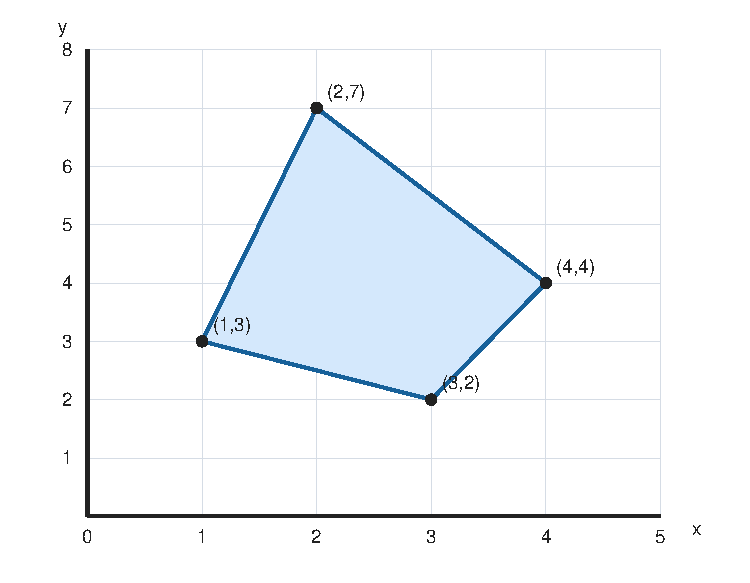
\includegraphics[width=0.56\linewidth]{recursos/figuras/s016-region.pdf}\end{center}
En esos vértices, $F=2x+y$ vale $5$, $8$, $12$ y $11$. Por tanto,
\[
\boxed{F_{\min}=5\text{, únicamente en }(1,3).}
\]
Comprobación global:
\[
2x+y=\frac23(x+2y)+\frac13(4x-y)\geq\frac{14+1}{3}=5.
\]
La igualdad fuerza las dos primeras fronteras y determina ese punto.
